% begin module differentiable-ex5
\begin{frame}[t]
\begin{example} %[Example 6, p. 150]
Where is the function $f(x) = |x|$ differentiable?
\begin{columns}[c]
\column{.25\textwidth}
\
\psset{xunit=0.75cm, yunit=0.75cm}
\begin{pspicture}(-2,-2)(2,2)
\psframe*[linecolor=white](-2,-2)(2,2)
\psaxes[ticks=none, labels=none]{<->}(0,0)(-2,-2)(2,2)
\tiny
\psLabelXOne
\psLabelYOne
\rput[t](1.3, 0.7){$y=f(x)$}
%Function formula: x 
\psplot[linecolor=red, plotpoints=1000]{0}{2}{x} %Function formula: - (x) 
\psplot[linecolor=red, plotpoints=1000]{-2}{0}{x -1 mul }
\end{pspicture} 
%\ 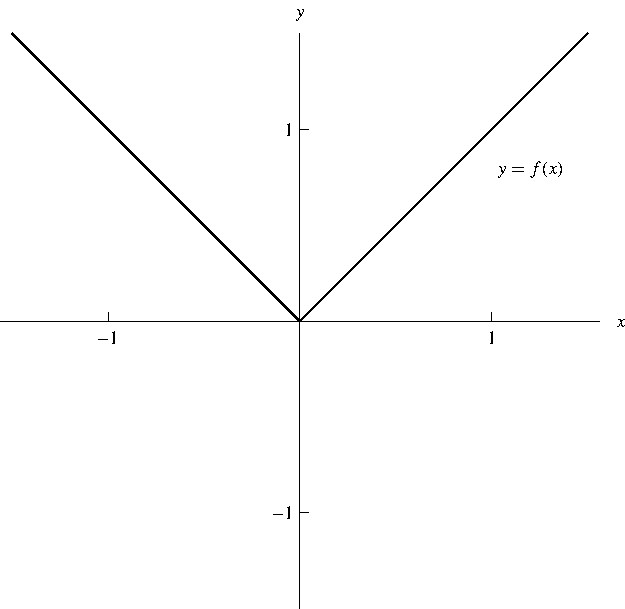
\includegraphics[height=3cm]{derivatives/pictures/03-02-ex5a.pdf}%
%\ \only<handout:-2| -30>{%
%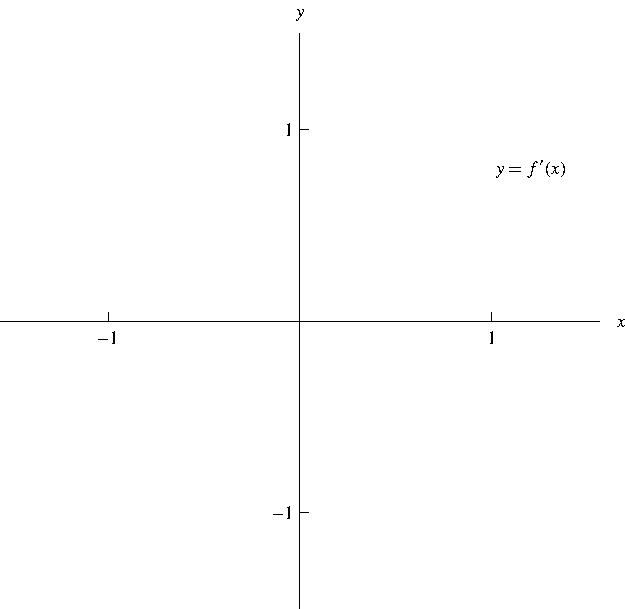
\includegraphics[height=3cm]{derivatives/pictures/03-02-ex5b.pdf}%
%}%
%\only<handout:3| 31->{%
%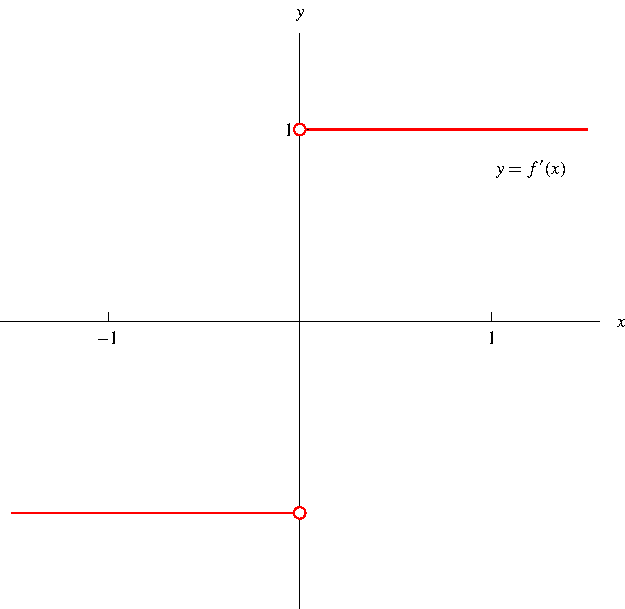
\includegraphics[height=3cm]{derivatives/pictures/03-02-ex5c.pdf}%
%}%
\psset{xunit=0.75cm, yunit=0.75cm}
\begin{pspicture}(-2,-2)(2,2)
\psframe*[linecolor=white](-2,-2)(2,2)
\psaxes[ticks=none, labels=none]{<->}(0,0)(-2,-2)(2,2)
\tiny
\psLabelXOne
\psLabelYOne
\uncover<31->{
%Function formula: 1 
\psplot[linecolor=blue, plotpoints=1000]{0}{2}{1} %Function formula: -1 
\psplot[linecolor=blue, plotpoints=1000]{-2}{0}{-1}
\psHollowDotBlue{0}{1}
\psHollowDotBlue{0}{-1}
\rput[b](1.2, 1.1){$y=f'(x)$}
}
\end{pspicture} 
\vspace{0.1cm}
\column{.75\textwidth}
\only<handout:1| -10>{%
\begin{itemize}
\item<2->  Suppose $x > 0$.
\item<3-| alert@7>  Then $|x| = x$.
\item<4->  If $|h|<x$ it follows that $x + h > 0$.
\item<5-| alert@7>  Then for $|h|<x$ we have $|x + h| = x+h$.
\end{itemize}
\abovedisplayskip=0pt
\belowdisplayskip=0pt
\begin{align*}
\uncover<6->{f'(x)}%
 & \uncover<6->{ = } %
\uncover<6->{\lim_{h\rightarrow 0} \frac{|x+h|-|x|}{h}}\\%
 & \uncover<7->{ = } %
\uncover<7->{\lim_{h\rightarrow 0} \frac{(x+h)-x}{h}}\\%
 & \uncover<8->{ = } %
\uncover<8->{\lim_{h\rightarrow 0} \frac{h}{h}}\uncover<9->{ = 1}%
\end{align*}
\uncover<10->{%
Therefore $f$ is differentiable for any $x > 0$.
}%
}%

\only<handout:2| 11-19>{%
\begin{itemize}
\item<11->  Suppose $x < 0$.
\item<12-| alert@16>  Then $|x| = -x$.
\item<13->  If $|h|<|x|$ it follows that $x + h < 0$.
\item<14-| alert@16>  Then $|x + h| = -(x+h)$.
\end{itemize}
\abovedisplayskip=0pt
\belowdisplayskip=0pt
\begin{align*}
\uncover<15->{f'(x)}%
 & \uncover<15->{ = } %
\uncover<15->{\lim_{h\rightarrow 0} \frac{|x+h|-|x|}{h}}\\%
 & \uncover<16->{ = } %
\uncover<16->{\lim_{h\rightarrow 0} \frac{-(x+h)+x}{h}}\\%
 & \uncover<17->{ = } %
\uncover<17->{\lim_{h\rightarrow 0} \frac{-h}{h}}\uncover<18->{ = -1}%
\end{align*}
\uncover<19->{%
Therefore $f$ is differentiable for any $x < 0$.
}%
}%


\only<handout:3| 20->{%
If $f'(0)$ exists, then 
\[
f'(0) = \lim_{h\rightarrow 0}\frac{f(0+h) - f(0)}{h} = \lim_{h\rightarrow 0} \frac{|0+h| - |0|}{h}.
\]
\uncover<21->{%
Does this limit exist?
}%
\abovedisplayskip=0pt
\belowdisplayskip=0pt
\[
\uncover<22->{%
\lim_{h\rightarrow 0^{\alert<handout:0| 24>{+}}}\frac{|0+h|-|0|}{h}
}%
\uncover<23->{%
 = \lim_{h\rightarrow 0^{\alert<handout:0| 24>{+}}}\frac{\alert<handout:0| 24>{|h|}}{h}
}%
\uncover<24->{%
 = \lim_{h\rightarrow 0^{\alert<handout:0| 24>{+}}}\frac{\alert<handout:0| 24>{h}}{h}
}%
\uncover<25->{%
 = 1
}%
\]
\abovedisplayskip=0pt
\belowdisplayskip=0pt
\[
\uncover<26->{%
\lim_{h\rightarrow 0^{\alert<handout:0| 28>{-}}}\frac{|0+h|-|0|}{h}
}%
\uncover<27->{%
 = \lim_{h\rightarrow 0^{\alert<handout:0| 28>{-}}}\frac{\alert<handout:0| 28>{|h|}}{h}
}%
\uncover<28->{%
 = \lim_{h\rightarrow 0^{\alert<handout:0| 28>{-}}}\frac{\alert<handout:0| 28>{-h}}{h}
}%
\uncover<29->{%
 = -1
}%
\]
\uncover<30->{%
Therefore $f$ is not differentiable at $0$.
}%
\uncover<31->{%
\abovedisplayskip=0pt
\belowdisplayskip=0pt
\[
f'(x) = \left\{ \begin{array}{rl}
1 & \text{ if } x > 0\\
-1 & \text{ if } x < 0\\
\end{array}\right.
\]
}%
}%
\end{columns}
\end{example}
\end{frame}
% end module differentiable-ex5
